\documentclass{article}

\usepackage[most]{tcolorbox}
\usepackage{physics}
\usepackage{graphicx}
\usepackage{float}
\usepackage{amsmath}
\usepackage{amssymb}


\usepackage[utf8]{inputenc}
\usepackage[a4paper, margin=1in]{geometry} % Controla los márgenes
\usepackage{titling}

\title{Clase Agujeros Negros Cuánticos }
\author{Manuel Garcia.}
\date{\today}

\renewcommand{\maketitlehooka}{%
  \centering
  \vspace*{0.05cm} % Espacio vertical antes del título
}

\renewcommand{\maketitlehookd}{%
  \vspace*{2cm} % Espacio vertical después de la fecha
}

\newcommand{\caja}[3]{%
  \begin{tcolorbox}[colback=#1!5!white,colframe=#1!25!black,title=#2]
    #3
  \end{tcolorbox}%
}

\begin{document}
\maketitle

\section{Formulación Clásica }
\begin{figure}[H]
  \begin{center}
    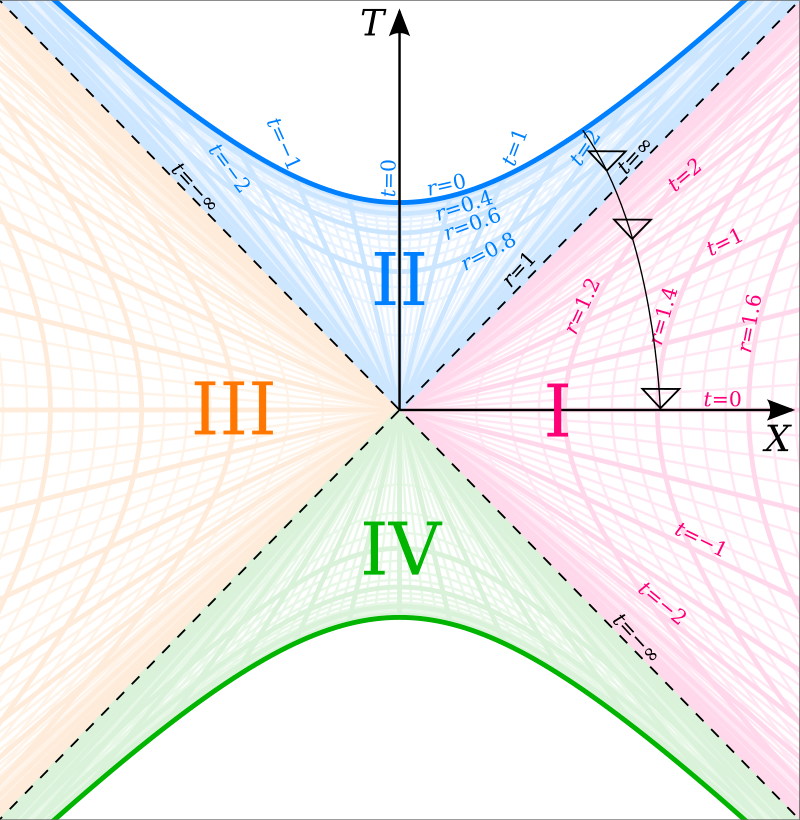
\includegraphics[width=0.35\textwidth]{kruskal.png }
  \end{center}
\end{figure}
Considérese un campo escalar real $ \phi  $ definido sobre Kruskal. 

En lenguaje genérico, para las regiones I y II la métrica se expresa como: 
\begin{gather*}
  ds^2 = g _{00 } dt^2 + g _{ab }  dx^a dx^b  \qquad \qquad \text{donde }g _{00 }  = - f(r)
\end{gather*}

Podemos escribir el Lagrangiano para acople minimal: 
\begin{gather*}
  \mathcal L (x) = \frac{1}{2} [-g(x)]^ {1/2 } \{g ^ {\mu\nu}(x) \phi(x)_{'\mu} \phi(x)_{'\nu} - m^2 \phi^2(x)\} 
\end{gather*}
Donde $ \phi _{'\mu} = \frac{\partial \phi  }{\partial x^\mu}  $

\hfill

La acción: 
\begin{gather*}
  S = \displaystyle\int_{}^{} \mathcal L (x) d^4 x \\
  \delta S = 0 \\
  [\Box - m^2 ] \phi(x) = 0 
\end{gather*}
Esta es la ecuación de Klein-Gordon que funciona para el caso de partículas escalares o con spin 0.

Donde el operados D'Alambertiano está definido como:
\begin{gather*}
  \Box := (-g)^ {1/2 } \partial_0 [(-g)^ {1/2 } g ^ {00 } \partial_0 ] +  (-g)^ {1/2 } \partial_a [(-g)^ {1/2 } g ^ {ab } \partial_b ]
\end{gather*}

\hfill 

Un conjunto de modos de solución de la ecuación de Klein-Gordon para $ R   $
\begin{gather*}
  \phi _\Omega (t,x) = \phi_\Omega Y _{lm } (\theta, \phi ) \frac{1}{\sqrt{2 \left|\omega\right|} } e ^ {-i \omega t }
\end{gather*}
Donde $ \Omega = \omega l m  $ y $ l  $ es el momento angulas orbital y $ m  $ el numero cuántico magnético orbital. 

\end{document}
